\documentclass[nonacm,sigplan,review]{acmart}

\renewcommand\footnotetextcopyrightpermission[1]{}
\settopmatter{printfolios=false,printacmref=false}

\usepackage{setspace}
\usepackage{enumerate}
\usepackage{algorithm2e}
\usepackage{algpseudocode}
\usepackage{graphics}
\usepackage{xparse} 
\usepackage{xspace}
\usepackage{multirow}
\usepackage{csvsimple}
\usepackage{balance}
\usepackage[newfloat]{minted}
\usepackage{xcolor}
\usepackage{nicefrac}
\usepackage{siunitx}
\usepackage{array,framed}
\usepackage{booktabs}
\usepackage{color}
\usepackage{soul}
\usepackage{float}
\usepackage{epsfig}
\usepackage{wrapfig}
\usepackage{graphics}
\usepackage{graphicx}
\usepackage{subcaption}
\usepackage{adjustbox}
\usepackage{csquotes}
\usepackage{cleveref}
\usepackage{dirtytalk}
\usepackage{textgreek}
\usepackage{oplotsymbl}
\usepackage{listings}
\usepackage{flushend}
\usepackage{float}
\usepackage{algorithm2e}

\def\eg{{\em e.g.}, }
\def\ie{{\em i.e.}, }
\def\etc{{\em etc.}\xspace}
\def\vs{{\em vs.}\xspace}

\def\gptmodel{{GPT-4o}\xspace}

\newcommand{\todo}[1]{\hl{\textbf{TODO:} #1}\xspace}
\newcommand{\sys}{{\scshape Kv{$\alpha$}sir}\xspace}
\newcommand{\rf}[1]{\ref{#1}}
\newcommand{\sx}[1]{(\S\ref{#1})}
\newcommand{\cf}[1]{(\emph{Cf}.\S\ref{#1})}
\newcommand{\se}[1]{\S\ref{#1}}
\newcommand{\fg}[1]{Fig.~\ref{#1}}
\newcommand{\heading}[1]{\vspace{2pt}\noindent\textbf{\emph{#1}}:\enspace}
\newcommand{\ttt}[1]{\texttt{#1}\xspace}
\newcommand{\xxx}{\colorbox{red!30}{xxx}\xspace}
\newcommand{\promptbox}[1]{%
  \vspace{0.5em}%
  \hspace*{-0.0135\columnwidth}%
  \fbox{%
    \parbox[t]{0.95\columnwidth}{\tt #1}%
  }%
  \vspace{0.5em} % adjust this value as desired
}

\crefformat{section}{\S#2#1#3}
\crefmultiformat{section}{\S#2#1#3}{--\S#2#1#3}{, \S#2#1#3}{ and \S#2#1#3}

\begin{document}


\title[Property-Guided Program Regeneration]{\sys: Property-Guided Program Regeneration\\{\vspace{1em}\large Technical University of Denmark, MSc Thesis {\\\vspace{-1em}} Advisors: Christian Gram Kahlauge and Nikos Vasilakis}}
\author{Evangelos Lamprou}


% Use cases for something like this include:
% - program repair
% - turning insecure code into secure code by removing side-effects
% - transforming a program in language A to language B
% - turning a program into a more idiomatic version of the same language
% - having a program use a different API
% - have a program be more amendable to parallelization
% - have a program be more amendable to further analysis or transformation

\begin{abstract}
  Software evolution tasks---like security hardening, porting critical components to safer 
  languages, or refactoring opaque legacy code---are brittle and time-consuming.
  Large language models (LLMs) have shown promise in automating such tasks,
  but their outputs are shaped by surface cues, lack
  semantic guarantees, and their usage often boil down to fragile prompting strategies.
This work presents \sys, a system for controllable program regeneration that
  combines declarative property constraints with LLM-guided synthesis. Unlike
  prior approaches, \sys treats the input program as an untrusted artifact and
  explicitly projects it into a set of verifiable properties, such as
  input/output behavior, execution traces, and API signatures. These properties
  serve as constraints during synthesis, are checked post hoc to ensure
  correctness, and can be mutated to allow for flexible program transformation through regeneration.
\sys is evaluated on a diverse set of program transformation tasks
including security hardening, language translation, idiomatic rewriting, de-obfuscation,
and modular refactoring showing strong results, even on tasks where state-of-the-art LLMs fail.
\end{abstract}
\maketitle

\section{Introduction}
\begin{figure}[t]
  % https://docs.google.com/drawings/d/1LAmdVYjfAID24eSM-hl5PRhVg9fRMJMWYETsvvcyAuU/edit?usp=sharing
  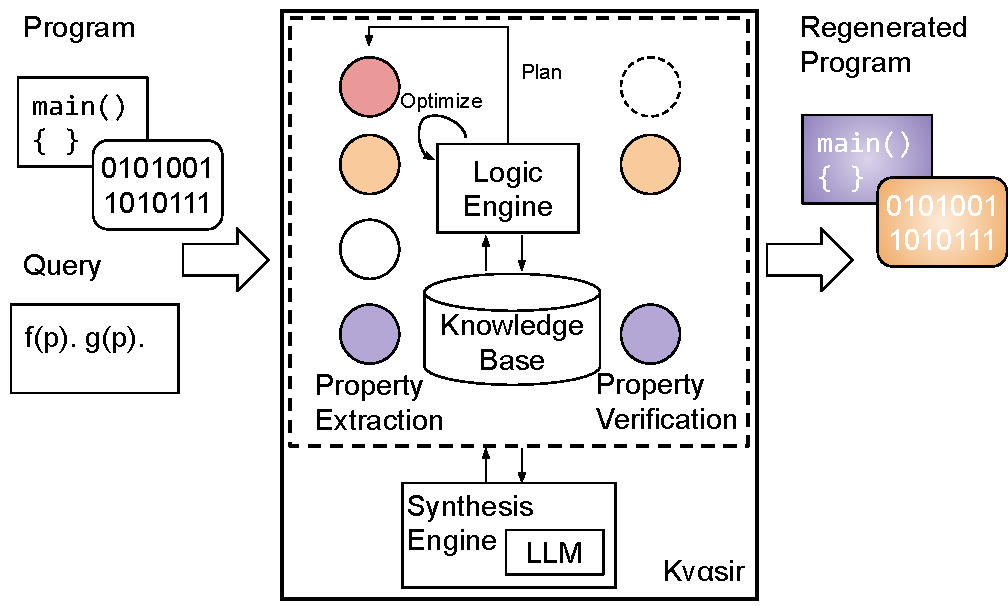
\includegraphics[width=.9\columnwidth]{figs/kvasir_overview.pdf}
  \caption{\textbf{\sys overview}
Given a transformation query, and a source program, \sys extracts a set
  of properties,
  guided by a logic engine and knowledge base.
  It then synthesizes a new program $P'$ that satisfies the query, verifying
  that wanted properties are present and unwanted properties are absent in $P'$.
}
  \label{fig:overview}
\end{figure}


% insights: modular programs, advances in LLMs, need for a strictly declarative interface

% Mention that:
% 1. They have shown great promise in program synthesis + 
% 2. They can not do negative reasoning well - 
% 3. Their output are often closely aligned to their inputs. They are gullible (susceptible to adversarial inputs). -
% 4. Difficult to verify correctness of outputs against certain properties. The
%    user cannot easily set requirements or say output should be within a range of
%    acceptance


Modern software systems evolve constantly.
Developers refactor legacy code~\cite{Fowler99,Mens04,facebook2010redesigns,dropbox2014syncengine},
adapt libraries to changing APIs~\cite{dig2005role,kula2017empiricalstudyimpactrefactoring},
translate components across languages~\cite{manzoor_cli_python,gaultier_rewrite_cpp},
and patch security vulnerabilities~\cite{ikegami2022userefactoringsecurityvulnerability,schneier2013security_vulnerabilities}.
These transformations, are often brittle, time-consuming, and require significant expertise.

Recent advances in large language models (LLMs) have opened new possibilities for automating program transformation and synthesis tasks, making them attractive tools for software evolution, albeit with caveats.
This flexibility makes LLMs more attractive for software evolution than traditional synthesis techniques, which struggle to scale or generalize
across languages and domains~\cite{reynolds2019syguscomp,leino2016dafny,wu2023programming,dynamoth2016,cambronero2019active}.
LLMs can translate code across languages~\cite{ou2025enhancingllmbasedcodetranslation},
refactor complex modules~\cite{ziftci2025migrating},
and even generate entire components from scratch~\cite{huynh2025largelanguagemodelscode}.
However, surface-level patterns in the input shape their outputs~\cite{yang2025evaluatinggeneralizationcapabilitieslarge},
they struggle with negative constraints~\cite{hwang2024thinkpinkelephant,jiang2024llmsdreamelephantswhen},
often overfit to spurious input cues~\cite{xu2023llmfoolitselfpromptbased, wu2023deceptpromptexploitingllmdrivencode},
and lack mechanisms for enforcing precise behavioral properties on the generated code~\cite{roh2025breakthechainreasoningfailuresllms}.
As a result, developers must prompt and steer them through brittle heuristics or manual trial-and-error, leading to workflows that are difficult to audit, integrate, or systematically reason about.
Bridging this gap calls for a declarative interface---one that allows developers to specify explicit semantic constraints and transformation goals, and to reason about their satisfaction in a principled way.

This work presents \sys, a system for \emph{property-guided program regeneration}.
\sys allows users
to express transformation goals declaratively, as logical constraints over
program properties such as input/output behavior, side-effect freedom, target
language, trace equivalence, or modular structure.
As shown in \cref{fig:overview}, given a source program and
a query, \sys extracts a set of relevant properties, guided by its
logic engine, and synthesizes a new
program that satisfies the given constraints.

Three key insights shape the design of \sys.
First, modern software is highly modular, making it feasible to reason about transformations at the granularity of individual components or functions.
Second, the program regeneration setting provides a unique advantage: the original program serves as a concrete ground-truth, enabling semantic comparisons and verification of the transformed output, something impossible in traditional synthesis tasks.
Third, the underlying synthesis technology---particularly LLMs---is evolving rapidly; a declarative interface that harnesses this progress without disrupting the framework's end user.

Guided by these insights, \sys casts transformation as a constrained synthesis problem.
At its core is a property-driven pipeline: users express goals as logical constraints over semantic properties, such as input/output behavior, side-effect freedom, target language, or structural modularity.
\sys extracts a set of relevant properties, derived from its logic engine and a domain-aware knowledge base, and synthesizes a new program that satisfies the specified constraints.
If no such program exists, \sys returns a failure explanation from the unsatisfiable core.

\heading{Deployment scenarios and limitations}
\sys supports a range of deployment scenarios.
It is particularly well-suited for use during maintenance and auditing phases, where developers seek to refactor or replace components, especially when the original code is difficult to understand, modify, or is unavailable and the component exists only as a binary.
It can also assist during development, for instance when integrating third-party modules that must be adapted to local conventions or hardened against security vulnerabilities.
However, \sys is not designed for whole-program synthesis or large-scale migrations.
Its strength lies in scoped regeneration tasks, typically at the granularity of a function, method, or small module---where transformation goals can be explicitly stated and verified in isolation.
To this end, \sys functions not only as a standalone tool but also as a
library, where other components can invoke it as a programmable,
constraint-guided regeneration module.

% Leverages insights: (1) modern applications highly modular (2) the problem of LLM-assisted program transformations needs to be transformed in a way that a ground truth is readily available: the original program
% (3) towards the generality and longevity of this solution the interface needs to be purely declarative, to allow independent progress of the underlying components to give automatic benefits

% TODO: Add section references
\heading{Contributions}
This work's contributions are:
\begin{itemize}
 \item A program transformation framework the combines logic-based reasoning with LLM-assisted program synthesis~(\cref{sec:design});
 \item A declarative interface and accompanying DSL for program transformation, allowing users to express semantic goals as logical queries over properties of the regenerated program~(\cref{sec:dsl});
 \item A verification architecture that checks synthesized programs against the specified properties, providing feedback for refinement~(\cref{sec:verification});
 \item An empirical evaluation demonstrating \sys's effectiveness and scalability across transformation scenarios~(\cref{sec:evaluation}).
\end{itemize}

\sys is evaluated across a diverse set of transformation tasks~(\cref{sec:evaluation}), including:
	security hardening, by stripping latent malicious behavior while preserving intended functionality;
	cross-language translation, by regenerating semantically equivalent programs in new languages;
	idiomatic rewriting, by producing safer and more portable variants of legacy code;
	modular decomposition, by restructuring monolithic components into composable parts.
\sys is able to effectively regenerate programs across these tasks, producing high-quality outputs that satisfy user-specified constraints while also discovering transformation strategies that were not immediately obvious to the authors.

\heading{Availability}
The \sys prototype in available as an open-source MIT-licensed artifact at:
\begin{center}
  \url{https://github.com/vagos/kvasir}
\end{center}

\section{Example}
\label{sec:example}

Given a program and a query over desired properties,
\sys selects a set
of properties to extract from the original program, then attempts to synthesize
a new program that satisfies the query.
\sys casts this process as an optimization problem, where the goal is to find a
program that satisfies the query.
If the query is unsatisfiable under
the constraints or transformations, \sys issues an error
message, showing the conflict.

This section shows the application of \sys
to four distinct program transformation tasks, 
targeting security,
language translation,
idiomaticity,
and modularity.

A user applying \sys would issue the following commands that 
take as input a query (\ttt{-q}), an input file parametrized parametrized over its line numbers (\ttt{-i}), and an output file (\ttt{-o}).
\begin{minted}{shell}
$ kvasir -q qp.pl -i flatmap.js -o flatmap.hs
$ kvasir -q qi.pl -i physics.c:10-27 -o physics.c
$ kvasir -q qm.pl -i app.js:1-30 -o app.js
\end{minted}

\heading{A compromised javascript library}
The \ttt{flatmap-stream} library was implicated in a high-profile
supply-chain attack that exfiltrated Bitcoin credentials~\cite{ev:eurosec:2022}.
While the library preserved
its client-observable behavior, an malicious payload inserted in the module's code by an adversarial developer accessed the filesystem, network, and
global state under specific conditions.
Speficially, 
the library would
(1) detect whether it is running under the dependency tree of a popular bitcoin wallet
application~\cite{copay} and on the live bitcoin network,
(2) collect the user's private keys, 
(3) send those to an attacker-controlled machine,
and finally (4) perform its benign functionality.
Program regeneration can automatically remove such malicious payloads
using the insight that the insight that they retain the original library's functionality,
while performing a side-effectful attack on-the-side~\cite{harp:ccs:2021}.
This approach can secure the component even when the attack is highly obfuscated and 
activates under precise conditions.
The slightly simplified source code of the compromised library showing the malicious payload and a final
line that performs the benign flatmap functionality is shown below:
\begin{minted}[frame=lines]{js}
module.exports = function (stream, fn) {
 if (process.env.PRODUCTION) {
  const priv = copay.getKeys()?.[0]?.priv;
  if (priv && wallet.balance > 0) {
    http.request({ hostname: 'evil.com' })
        .send({ priv });
  }} return flatten(steam).apply(fn); };
\end{minted}

\begin{wrapfigure}[4]{r}{.7\columnwidth}
\vspace{-10pt}
\hspace{-10pt}
\begin{minted}{prolog}
graph(p_, I, O) :- graph(p, I, O).
fsignt(p_, S) :- fsignt(p, S).
pure(p_).
\end{minted}
\end{wrapfigure}
To the right is a program written in the \sys query language to express 
this regeneration goal.
This query requires the regenerated program \ttt{p\_} to exhibit the same I/O behavior as the original program \ttt{p}
but forbids side-effects.
\sys takes this query and arrives at the set of properties to extract from the
original program, given its knowledge base and the query.
This set is $\{$\ttt{graph(p, I, O)}, \ttt{inpt(P, I)}, \ttt{fsignt(P, S)}, \ttt{pure(P)}$\}$, where
\ttt{input(p, I)} means that \sys will use the \ttt{input} plugin extract a set of inputs from the original program
by providing the program's source code to an LLM instance and asking it to generate a set of inputs;
\ttt{graph(p, I, O)} extracts the client-observable I/O behavior of the program
by executing the original program on the generated inputs and recording the outputs
(an example I/O pair is $\langle\ttt{([1,[2,3]], (x)=>x+1)}\to\ttt{[2,3,4]}\rangle$);
and \ttt{fsignt(p, S)} extracts the function's signature using a language-aware parser.
The, \ttt{pure(p)} property means that \sys will not provide to the LLM 
instance any information that could encode side-effects, such as the
program's source code, a system call trace, or a filesystem access trace.
After 30.4 seconds and one attempt, having generated 30 I/O pairs, \sys generates the following program:
\begin{minted}[frame=lines]{js}
module.exports = function(stream, fn) {
  return stream.map(fn); };
\end{minted}

Building on the same source, \sys can perform cross-language
translation. 
Here, the goal is to regenerate a semantically equivalent version
of \ttt{flatmap-stream} in Haskell, to enable integration with a
Haskell-based pipeline or facilitate formal reasoning.

\begin{wrapfigure}[7]{r}{.5\columnwidth}
% \vspace{-10pt}
\begin{minted}{prolog}
graph(p_, Ih, Oh) 
  :- graph(p, Ijs, Ojs),
     tr(Ijs, Ih),
     tr(Ojs, Oh).
language(p_, haskell).
\end{minted}
\end{wrapfigure}
The query asks \sys to preserve I/O behavior and translate the input program to Haskell.
The \ttt{tr} predicate is a generic LLM-assisted translator, and in the query
converts the input/output examples from Javascript to Haskell.
In this case, the given query is sufficient for the translation to succeed, 
but a natural-language description of the transformation can be passed as an additional 
argument to \ttt{tr}.
\sys, same as before, extracts an I/O trace from the original program.
Then, it transforms each extracted I/O example into an equivalent one in Haskell (\eg 
the pair $\langle\ttt{([1,[2,3]], (x)=>x+1)}\to\ttt{[2,3,4]}\rangle$ 
becomes $\langle(\ttt{[1, [2,3]], Js("(x)=>x+1"))}\to\ttt{[2,3,4]}\rangle$).
Finally, it provides the transformed examples to a new LLM instance, prompting it
to generate a Haskell program that satisfies the same I/O behavior.
After 32.2 seconds, having generated and subsequently translated 20 I/O pairs,
\sys produces the following Haskell program (truncated for brevity):
\begin{minted}[frame=lines]{haskell}
flatmap :: (a -> b) -> NestedList a -> [b]
flatmap f (Elem x) = [f x]
flatmap f (List x) = concatMap (flatmap f) x
\end{minted}

\heading{An unidiomatic c program}
The fast inverse square root routine from the Quake III
engine~\cite{fast_inv_sqrt}
is a classic example of performance-oriented low-level programming.
The original implementation exploits type punning to manipulate IEEE
floats at the bit level---an optimization that relies on undefined behavior:

\begin{minted}[frame=lines]{c}
float Q_rsqrt(float number) {
 long i; float x2, y;
 const float threehalfs = 1.5F;
 x2 = number * 0.5F; y  = number;
 i  = * ( long * ) &y; // evil bit level hack
 i  = 0x5f3759df - ( i >> 1 );
 y  = * ( float * ) &i;
 y  = y * ( threehalfs - ( x2 * y * y ) );
 return y; }
\end{minted}

The following query for \sys uses lines-of-code a coarse metric of
idiomaticity. \sys will regenerate the program, minimizing this metric, while
preserving its I/O behavior.
\begin{wrapfigure}[3]{r}{.7\columnwidth}
  \vspace{-5pt}
  \begin{minted}{prolog}
graph(p_, I, O) :- graph(p, I, O).
#min N: len(p_, N).
  \end{minted}
\end{wrapfigure}
\sys extracts the set of properties \ttt{signature(F)} and \ttt{graph(F)} from
the original program, where \ttt{signature(F)} is the
signature of the function (including its name, return type, and arguments), and \ttt{graph(F)} is the I/O behavior of the function
on a set of generated inputs.
In this case, where the goal is to optimize an aspect of the program, \sys will re-prompt
the model to regenerate the program until it can make no improvements or there is a negligible difference after two consecutive iterations.
After 15.2 seconds, and two iterations, \sys produces the following program:
\begin{minted}[frame=lines]{c}
#include <math.h>
float Q_rsqrt(float number) {
    return 1.0f / sqrtf(number); }
\end{minted}
The regenerated version is easier to verify, portable across compilers, and
avoids undefined behavior.
A user could have also provided performance requirements using 
the \ttt{time(P)} property to further guide the regeneration process.
In this case, \sys would have run the two functions inside a tight loop and 
would have aborted the regeneration process if the performance of the generated
program was not within an acceptable user-defined threshold.

\heading{A rigid music application}
Consider a JavaScript application that retrieves and displays a user's music
collection from an SQLite database~\cite{codewithsadeemusicplayer, beets}:

\begin{minted}[frame=lines]{js}
function getAlbumsByArtist(artist) {
  const db = new Database("music.db");
  const rows = db.prepare("SELECT album
  FROM songs WHERE artist = ?").all(artist);
  return rows.map(row => row.album); }
\end{minted}

\begin{wrapfigure}[7]{r}{.7\columnwidth}
  \begin{minted}{prolog}
db("music.db").func(f1).func(f2).
trc_sql(p_,I,T) :-
   trc_sql(p,I,T), graph(p,I,_).
graph(call(f2,call(f1),I),I,O):-
                   graph(p,I,O).
\end{minted}
\end{wrapfigure}
Having the database initialization being in the same function as 
the database access has negative architectural and performance implications.
In addition, there exist systems that can benefit from further decomposition
of an application towards automatic distribution, parallelization or security~\cite{Towards_Modern_Ghemaw_2023, vasilakis2019ignis, vasilakis2018breakapp}.
The query above first specifies \ttt{music.db} as the database to use.
This information is relevant to the \ttt{trc\_sql} plugin, which records the SQL queries 
sent to the databse when the function is driven by an input $i$.
The set of inputs $I$ the function will be driven by is generated by the \ttt{graph} plugin.
An example of an input, SQL-trace pair is
$\langle\ttt{'Metalica'}$, $\langle$\ttt{SELECT album FROM songs WHERE artist = 'Metalica'}, \ttt{['Master of Puppets', 'Ride the Lightning']}$\rangle\rangle$,
which means that the input \ttt{'Metalica'} causes the resulting SQL query to be executed by the function,
which together with the resulting rows is the SQL trace.
The built-in \ttt{call} predicate redefines the structure of the program to be regenerated. 
Spefically, the query asks \sys to generate two functions such 
that the graph of the composition of the two is equivalent to the graph (and SQL trace) of the original program.
This transforms each I/O pair to (for example) $\langle\ttt{(f2(f1(), 'Metalica'))}, \ttt{[...]}\rangle$.
\sys first generates 24 inputs, then wraps the node process with monitors that extract the SQL queries.
Then, it executes the original program on each input, recording the output and SQL traces.
Following, \sys transforms the I/O pairs and the SQL traces into a prompt template,
and prompts an LLM instance to generate two functions $f_1$ and $f_2$, which when composed would have the given behavior.
Their composition is then again driven by the same inputs and the SQL traces and outputs are recorded.
After 20.4 seconds and two attempts, \sys arrives at two functions $f_1$, and 
$f_2$, where their composition $f_2(f_1(), i)$,
is equivalent to the original \ttt{getAlbumsByArtist} function across each input $i$ in regards to its graph and SQL trace .
The user could have provided specific signatures and names for each 
function as an additional guiding property.
The resulting program is:
\begin{minted}[frame=lines]{js}
function f1() {
 const sqlite = require('sqlite');
 return sqlite.open({filename: 'music.db'});
}

function f2(db, artist) {
 const rows = await db.all("SELECT album
 FROM songs WHERE artist = ?", artist);
 return rows.map(row => row.album); 
}
\end{minted}

\heading{Key results}
\sys is able to be effectively applied to all the above transformation goals,
producing high-quality outputs that satisfy user-specified constraints.
A total
of six plugins (\ttt{input}, \ttt{graph}, \ttt{fsignt}, \ttt{pure}, \ttt{trace\_sql}, and \ttt{tr})
were required to perform the above transformations, each
contributing either a set of extracted and verified properties, or a
transformation, and a set of pre- and post-conditions that the logic engine
uses to construct the regeneration plan.

\section{Overall Design}
\label{sec:design}

% \sys is a system for program regeneration: given an input program and a set of
% behavioral, structural, or syntactic properties, it synthesizes a new program
% that satisfies a specified subset of those properties. The system treats
% regeneration as a goal-driven process, guided by explicit property
% specifications and a symbolic planner that structures the search space for a
% backend synthesizer.
At a high level, \sys operates in four phases: (1) plan construction, (2)
property extraction, (3) program synthesis, and (4) verification and feedback.
These phases interact through a shared representation of the program.

\heading{Plan construction}
First, each of the available plugins contributes a set of pre and post-conditions 
to the logic engine.
These describe what needs to hold for an analysis to be applicable to the given 
program and what properties \sys will preserve or transform after regeneration.
Then, the planning component accepts one or more user-provided regeneration goals (termed as the query).
The full set of rules and predicates are used to construct a logic program
which is then given to an off-the-shelf solver~\cite{gebser2007clasp}.
From the solver's output, the planner constructs a plan that specifies which
analyses \sys plugins should apply to the input program and what properties can be
preserved during regeneration in order to fulfill the query.
If the query is unsatisfiable, \sys halts and produces an error message.

\heading{Property extraction} \sys then continues by analyzing the input program to
extract the collection of properties.
These may describe the program's interface
(\eg, exported functions), its operational constraints (\eg, disallowing
filesystem access), or its structure (\eg, use of a particular API or programming idiom).
Some properties are derived from generic analyses
applicable across languages~(\eg input-output behavior) 
and others are specific to the input program's language and runtime model.
Plugins insert preconditions for the analyses they provide into the \sys knowledge base.

\heading{Synthesis}
Guided by the transformation plan, \sys creates a prompt template which it then
augments with the extracted properties, having them normalized to a human-readable text representation.
This prompt is then passed to an LLM instance.

\heading{Verification and feedback}
The final phase verifies that the
synthesized program satisfies the target properties.
If verification fails---due to a violated constraint---\sys uses this
failure as a signal to refine the plan or re-sample the synthesis step.
This forms a feedback loop: planning, synthesis, and verification interact until \sys
produces a satisfactory program or the system exhausts its search.

\section{Query Language}
\label{sec:dsl}

\sys represents program characteristics as symbolic \emph{properties}, drawn from a language of first-order predicates.
These properties describe aspects of the input program and serve as regeneration constraints for the output.
They form the basis of both planning and verification.
All aspects of the symbolic representation are expressed as logic facts and rules (an example program is shown in \cref{lst:logic-example}).

\begin{listing}[t]
  \begin{minted}[frame=lines, fontsize=\small]{prolog}
% Original query (q.pl)
graph(p_, Ih, Oh) :- graph(p, Ijs, Ojs),
    tr(Ijs, Ih),
    tr(Ojs, Oh).
language(p_, haskell).

% Compiled program
% Base program facts
program(p).
program(p_).
language(p, javascript).
% -----------
% Plugin-provided facts
can(graph(P)) :- language(P, javascript).
can(tr).
% ------------
% Query predicates
can(graph(P, graph_p_Ijs, graph_p_Ojs)) :-
    do(graph(P)),
    program(P).
% ...compilation of tr predicates...
can(language(P, haskell)) :-
    program(P).
% ------------
% Axioms
:- do(language(P, L1)), language(P, _). 
% ----------
% Regeneration plan choice rule
0 { do(X) } 1 :- can(X).
% User query goals
:- not do(graph(p_,tr_graph_p_Ijs_Ih,tr_graph_p_Ojs_Oh)).
:- not do(language(p_, haskell)).
#show do/1.
\end{minted}
  \caption{\textbf{Compiled \sys logic program.}
  The logic program that produces the plan for the idiomatization task in \cref{sec:example}. 
  The program contains facts coming from 
  (1) the input program (written in C),
  (2) three plugins (\ttt{len}, \ttt{fsignt}, and \ttt{tr}),
  (3) axioms from the logic engine (\eg a program can have one language, an analysis will be applied only if possible, all goals must be satisfied), and
  (4) the user query (the user wants to minimize the program's length).
  }
  \label{lst:logic-example}
\end{listing}

% To compute answer sets, ASP programs are input into ASP solvers.
% These solvers provide efficient mechanisms to generate the set of valid answers to the given problem.
% An ASP solver can be thought of as a black box, with them being interchangeable as 
% long as the input language semantics remain the same.



\heading{Property predicates}
Each property is a logical predicate over the program symbol $p$,
or a derivative symbol extracted from $p$.
For example, 
the \ttt{language}$(p, \ttt{javascript})$ predicate describes that the input program is written in JavaScript.
The \ttt{fsignt}$(p, S)$ predicate is used to extract well-formed function signature $S$ when the program \ttt{p} exposes one.
If the user wanted to refer to each function in the program, they could 
combine the predicates \ttt{func(F, p)} and \ttt{fsignt(F, S)} in a single rule in their query.
The \ttt{pure}$(p)$ predicate can be used as a contraint
to signify that the regenerate program
should not have side-effects (\eg file system access, network calls, \etc).

A property $X$ appears as either an
  plugin-provided $\mathsf{can}(X)$ atom, which denotes that the system is capable of extracting or inferring property $X$ from the input.
  A pure $X$ atom denotes that either the user has explicitly requested property $X$ to be enforced, or the planner has deduced that it is necessary to satisfy the query.

\sys also supports minimization, maximization and elimination of properties
through the $\mathsf{min}$, $\mathsf{max}$, and $\mathsf{not}$ directives.

\heading{Planning over properties}
The logic engine determines the set of active properties to enforce by solving
a constrained optimization problem over the extractable property set $P_r$.
It satisfies the
following key constraint:
\begin{align*}
  X &\Leftarrow \mathsf{can}(X) &\text{Apply only extractable properties}
\end{align*}

Additionally, the system takes advantage of ASP's least stable model semantics.
Intuitively, the planner tries to give the synthesizer the least amount of information
possible, as long as all regeneration goals are fulfilled.

\heading{Plugin-defined rules}
Plugins can also contribute domain-specific inference rules and constraints.
For example, a plugin for JavaScript-to-Haskell translation may define:
\begin{align*}
\mathsf{can}(\ttt{translate}_{\ttt{js} \rightarrow \ttt{hs}}(p)) & \\
\ttt{translate}_{\ttt{js} \rightarrow \ttt{hs}}(p) &\Rightarrow \ttt{language}(p, \ttt{haskell}) \\
\ttt{translate}_{\ttt{js} \rightarrow \ttt{hs}}(p) &\Rightarrow \mathsf{language}(p, \ttt{javascript})
\end{align*}
Intuitively, these rules mean (1) that the system is able to apply the plugin,
and (2) it can only be applied if the original program is written in JavaScript, 
and the regenerated program \emph{must} be written in Haskell.

\heading{Axioms and domain knowledge}
The logic engine also includes domain-wide axioms based on some common assumptions.
For example
$\ttt{language}(p, \ttt{haskell}) \Rightarrow \ttt{pure}(p)$
captures the assumption that programs written in Haskell are pure by default.
Such axioms allow inferred properties to trigger downstream constraints or synthesis behaviors.

\heading{Compilation to ASP}
Given a source program written in the \sys query language, the compiler
performs a syntactic de-sugaring into ASP rules~(\cref{fig:asp-compilation}).
For each rule $H \leftarrow B_1,\dots,B_n$, the compiler first performs a
pseudo-grounding step that replaces every capitalized variable $V_i$ with a
fresh, unique symbol $\mathit{sym}(r,P,V_i)$, generated from the rule
name $r$, target program $P$, and original variable name $V_i$, proceeding
left-to-right to preserve data dependencies.
Each one of these concrete values will correspond to extracted program properties.
After renaming, the head and body
are emitted as an ASP capability rule of the form $\mathit{can}(H') \leftarrow
\mathit{do}(B_1'),\dots,\mathit{do}(B_n')$. 
All implicit query
goals (rule heads $H$) are compiled into hard constraints $\neg \mathit{do}(H) \rightarrow
\bot$, meaning that the ASP program will be unsatisfiable unless all query goals are met.
Optimization directives $\#\min X$ and $\#\max X$ are mapped to
$\mathit{do_min}(X)$ and $\mathit{do_max}(X)$, respectively.
Finally, \sys
appends program-agnostic axioms and adds a choice rules that allows the solver to select which properties to extract from the program in order to satisfy the query.
This consists as the core of the \sys logic program, and the reason the rule to \ttt{can}/\ttt{do} predicates is required.
The result is the compilation is a valid ASP program which is then evaluated by an ASP solver.
The next section describes how the set of produced predicates is used to construct the regeneration plan.

\begin{figure}[t]
\centering
\small
\begin{tabular}{l}
\textbf{toasp} (q : Query) : ASPCode {$\leftarrow$} \textbf{match} q \textbf{with} \\[0.5ex]
  \quad \textbar~$p$: \textbf{program name} {$\rightarrow$} \ttt{program}$(p)$. \\[0.5ex]
  \quad \textbar~$X$: predicate {$\rightarrow$} \ttt{can}$(X)$ \\[0.5ex]
\quad \textbar~$H \leftarrow B_1,\dots,B_n$
    {$\rightarrow$} 
    $V_i$ 
    $\mapsto$ 
    $\mathit{sym}(r,P,V_i) = r\ttt{\_}P\ttt{\_}V_i$ \\
  \quad \textbar~$H \leftarrow B_1,\dots,B_n$ {$\rightarrow$} \ttt{can}$(H)$\ttt{ :- do}$(B_1)$, \dots, \ttt{do}$(B_n)$. \\[0.5ex]
  \quad \textbar~$H \leftarrow B$  {$\rightarrow$} \ttt{:- not do}$(H)$. \\[0.5ex]
  \quad \textbar~\#\ttt{min}~$X$ {$\rightarrow$} \ttt{do\_min}$(X)$. \\[0.5ex]
  \quad \textbar~\#\ttt{max}~$X$ {$\rightarrow$} \ttt{do\_max}$(X)$. \\[0.5ex]
\textbf{end} \\[1ex]
\multicolumn{1}{p{0.9\linewidth}}{\textit{Axioms and choice rules:}} \\[0.5ex]
\quad \ttt{0 \{ do(X) \} 1 :- can(X).} \\[0.5ex]
\quad \ttt{:- do(language(P,L1)), language(P,\_).} \\
\multicolumn{1}{p{0.9\linewidth}}{\textit{Plugin-supplied rules and facts.}} \\[0.5ex]
\end{tabular}
\caption{\sys query compilation into an ASP program.}
\label{fig:asp-compilation}
\end{figure}

\heading{Logic program resolution}
Once the input query is compiled into an ASP program, \sys invokes an
off-the-shelf ASP solver to compute a stable model that satisfies the query.
The model consists of a set of selected $\mathit{do}$ atoms representing the regeneration plan.
\sys then executes this plan~\cref{alg:resolution}.
First, \sys discards all plugin-activation atoms from the plan, 
as they are only relevant to the logic engine.
Then \sys iterates through each
$\mathit{do}(f(a_1,\dots,a_n))$ atom.
If an argument value is missing, the plugin responsible for producing
it (found by parsing the variable's name) is executed and produced program properties are stored in a value map.
Once all actions have been executed in dependency order, the extracted properties are passed to the regeneration phase.

\begin{algorithm}[t]
\caption{Resolution of a regeneration plan from an ASP model into concrete program-extracted values.}
\label{alg:resolution}
\DontPrintSemicolon
\SetKwInOut{Input}{Input}
\SetKwInOut{Output}{Output}
\Input{ASP model (set of \(\mathit{do}\) atoms)}
\Output{Map $V \mapsto V_p$ of concrete values for each property \(V\) in the model}
% initialize
\ttt{discard} all plugin‐activation atoms from \(\mathit{plan}\)\;
\(\mathit{values}\;\gets\;\emptyset\)\;
% main loop
\ForEach{\(d \in \mathit{plan}\)}{
  \If{\(d = \mathit{do}(f(a_1,\dots,a_n))\)}{
    \For{each argument \(a_i\) of \(f\)}{
      \If{\(a_i \notin \mathit{values}\)}{
        invoke plugin responsible for \(a_i\)\;
        \(\mathit{values}[a_i] \gets\) result of plugin\;
      }
    }
    invoke plugin \(f\) with \((a_1,\dots,a_n)\)\;
  }
}
\end{algorithm}

\heading{Logic and concrete space}
\sys operates at the boundary between two representational domains: a symbolic
\emph{logic space}, where transformations over program properties are expressed, and
a \emph{concrete space}, where actual programs, inputs, outputs, and traces
reside.

In the logic space, properties are encoded as predicates over abstract program
identifiers.
To bridge this abstraction gap, \sys given the set of true predicates
from the logic space, extracts the corresponding concrete properties from the
source program.
For example, the predicate $\ttt{inputs}(p, I)$ in the logic space
will be concertized to set of inputs $I$ by invoking the \ttt{input} plugin,
which uses an LLM to generate a set of inputs for the program $p$.
Similarly, the predicate $\ttt{graph}(p, I, O)$ will be concertized to a set of
input-output pairs $(I, O)$ by executing the program $p$ on the inputs $I$ and
recording the outputs $O$.
After regeneration, the predicates over the concrete regenerated program $p\_$
will be checked regarding their relationship to the same properties over program $p$
in the logic space.
% An equality relationship is one where the predicate's grounded version
% $X$ is the same between the two programs, modulo the program identifier~(\eg, $\ttt{graph}(p, i, o) \equiv \ttt{graph}(p\_, i, o)$).
Equality is defined differently for each property, and is enforced by the corresponding plugin.
Similarly, minimization and maximization relationships are defined as
the concrete property value being less-than or greater-than the original program's value, respectively.
Again, the less-than and greater-than operators are defined by the plugin that verifies the property.

% In the current \sys implementation, this translation is one-way,
% however the system can be extended to support two-way translation, where properties extracted
% can be used to generate new properties in the logic space.

As shown in \cref{fig:logic-to-concrete}, this process constitutes a
translation barrier: declarative goals over properties like \ttt{inputs},
\ttt{outputs}, and \ttt{traces} are realized through observation and
instrumentation. Once aligned, the logic engine can reason over these grounded
facts to drive transformation.

\begin{figure}[t]
\centering
  % https://docs.google.com/drawings/d/1JdOfgpaVUy7_EgFyguRXHxFKdmZwyHaiHshnifHG0TQ/edit?usp=sharing
  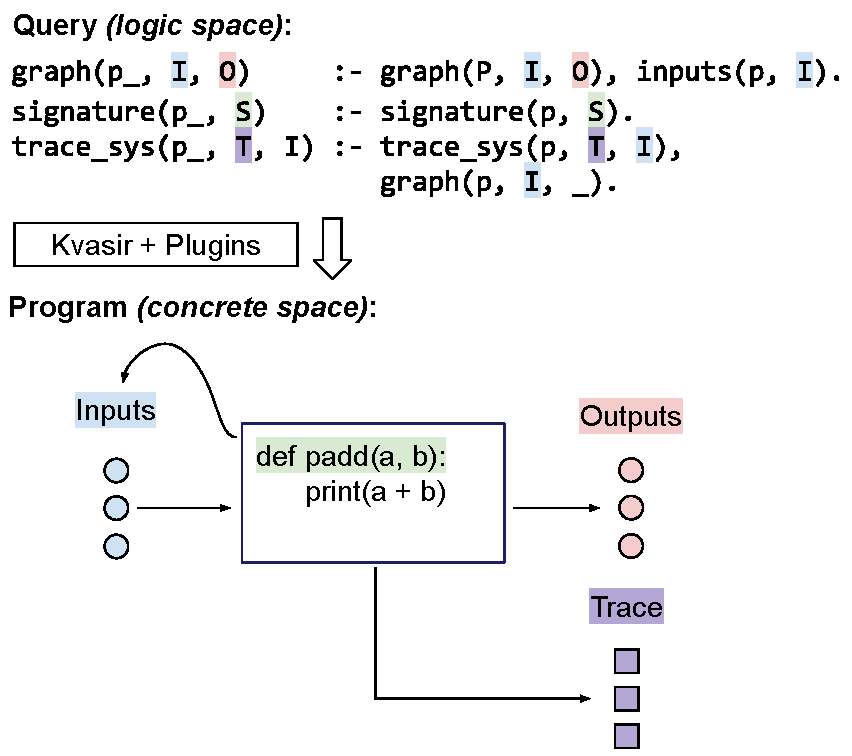
\includegraphics[width=.9\columnwidth]{figs/kvasir_logic-space.pdf}
  \caption{\textbf{\sys transforms a program over its properties from the abstract logic space to the concrete space.}
  Relationships between original and regenerated program's properties are inferred 
  from the query in combination with the knowledge base and enforced by \sys plugins.
  }
  \label{fig:logic-to-concrete}
\end{figure}


\heading{Extensibility}
\sys decentralizes property extraction: plugins contribute $\mathsf{can}(\cdot)$ facts, and pre- and post-conditions, while the core planner resolves which properties to enforce based on goals, capabilities, and axioms.
This allows many different types of analyses (language-aware, language-agnostic, or LLM-assisted)
to coexist in a unified planning layer.

\heading{Answer Set Programming}
The \sys prototype compiles each input query to an answer-set programming (ASP) program~\cite{Eiter_2009}.
A brief introduction to the paradigm follows.
ASP \cite{Gelfond_2000, Eiter_2009} is a problem-solving paradigm with roots in logic programming and non-monotonic reasoning.
The programming 
model of ASP is one where the programmer models
the problem domain, with the solution being handled by a solver program.
Programming using this paradigm is done in a family of languages sometimes called \textit{AnsProlog} \cite{Gelfond_2002}.
This work uses the input language of \textit{Clingo} \cite{DBLP:journals/corr/GebserKKS14}, which 
is a high-performance integrated solver with a large collection of libraries and bindings helpful in integrating it with external tools.

The syntax is similar to \textit{Prolog} and \textit{Datalog}, with code and data being represented
through logical terms.
Collections of logical terms, as seen in
\cref{lst:terms}, can represent the program and its properties.
Rules, expressed using
the \ttt{:-} operator, define relationships
between atoms.
Choice rules, exemplified in \cref{lst:choice}, allow the ASP
solver to make selections among atoms.
Integrity constraints, as shown in
\cref{lst:constraint}, can restrict invalid answer sets. Optimization
directives, such as \ttt{\#minimize} and \ttt{\#maximize} in
\cref{lst:optimization}, guide the solver to output optimal answer sets,
with respect to a given metric (\eg the number of properties to be extracted from the input program).

\begin{listing}
\begin{minted}{prolog}
language(p, javascript).
len(p, 100).
\end{minted}
\caption{A set of facts over a program.}
\label{lst:terms}
\end{listing}

\begin{listing}
\begin{minted}{prolog}
graph(p_) :- graph(p).
len(p_, N) :- len(p, N_), N = N_ + 1.
\end{minted}
\caption{Logic rules describing relationships between the original and regenerated program.}
\label{lst:rules}
\end{listing}

\begin{listing}
\begin{minted}{prolog}
{absent(F) : function(F, P)} :- program(P).
\end{minted}
\caption{A choice rule.}
\label{lst:choice}
\end{listing}

\begin{listing}
\begin{minted}{prolog}
:- language(p, X), language(p_, Y), X != Y.
\end{minted}
\caption{An integrity constraint.}
\label{lst:constraint}
\end{listing}

\begin{listing}
\begin{minted}{prolog}
#minimize{C : cost(E,C)}.
#maximize{C : cost(E,C)}.
\end{minted}
\caption{Examples of optimization directives. Note that this differs from \sys's \ttt{\#min} or \ttt{\#max} directives, which is used to direct the synthesizer to minimize a program's property but has no effect on the produced answer set.}
\label{lst:optimization}
\end{listing}


\section{Synthesis Plan}
\label{sec:synthesis}

The synthesis process begins with a set of enforced properties $\mathbf{X}$
which the planner selected~(\cref{sec:dsl}).
These properties
reflect both user goals (\eg removing side effects, translating to a
different language) and the input program's structural characteristics that
the synthesizer will preserve.
The planner constructs a transformation plan that
specifies, for each relevant unit of code (typically a function), what
constraints must hold in the regenerated version.

For instance, a plan for regenerating a specific function $f$ might include:
\ttt{language}(f, \ttt{haskell}) the function must be written in Haskell, 
\ttt{pure}(f)) the function must be side-effect-free, and 
\ttt{signature}(f, s)) the function must keep the original program's signature $s$.



\heading{LLM-guided regeneration}
A structured prompt guides the language model, which performs the synthesis task.
The prompt is a composition of natural-language text fragments plugins contribute. 
A plugin can include domain-specific instructions as further guidance.
For example:
A \ttt{signature} plugin may contribute:

 \promptbox{
   {The output should implement a function \ttt{sqrt(n: float): float}.}
 }
A \ttt{length} plugin combined with a minimization goal may prepend:

\promptbox{
  {The output should be as short as possible while preserving the original functionality.}
}
A \ttt{tr} plugin given that the output program must be written in Haskell, may prepend:

\promptbox{
  {The output function should be written in Haskell.}
}

These fragments, combined with a normalized text representations of each of 
the extracted properties constitute the prompt given to the LLM.

\heading{Constraint-guided generation}
While \sys delegates code synthesis to a large language model, the planner constrains the generation space in two key ways.
First, the prompt instructs the LLM to perform only transformations that are valid under the current plan.
For instance, if the target function must be pure, the prompt will exclude information such as system-call traces that might imply side-effectful behavior.
Second, candidate outputs are verified post hoc against the enforced properties~(\cref{sec:verification}).
% This hybrid model balances flexibility with rigor: the LLM provides diversity and fluency, while the planner ensures adherence to property-based constraints.

\section{Property Verification and Feedback Loop}
\label{sec:verification}

\sys includes an explicit verification phase that checks whether the output adheres to the enforced properties in the synthesis plan. 
Verification accepts only programs that meet the plan's constraints and
provides feedback for refining or retrying those that do not.
Checkers are contributed by plugins.

\heading{Verification as property checking}
After synthesis, \sys invokes a set of property-specific checkers.
Each checker
is responsible for evaluating whether a property $X$ holds
for the regenerated program fragment.
These checkers operate at varying levels
of precision---ranging from structural pattern checks to light static or
symbolic analysis.
Examples from the \sys prototype include:
  $\ttt{no\_network}(f)$, the checker confirms the absence of known network APIs or imports using static analysis~\cite{mir:ccs:2021};
  $\ttt{fsignt}(f)$, the checker matches the regenerated function's name, parameters, and arity against the extracted signature.

For minimization and maximization goals, the verification phase uses the less-than or greater-than operators as are defined internally by the verifier.
Verification in this case means if the property's value has decreased or increased compared 
to the previous regeneration attempt.
If the value remains unchanged for two consecutive attempts, its considered satisfied.

\heading{Failure-driven refinement}
When a candidate fails verification, \sys treats this as a feedback signal. Instead of discarding the regeneration attempt wholesale, the system uses the failure to revise or re-execute the synthesis phase.
\sys implements three strategies to handle regeneration failures:
  (1) \emph{retrying synthesis}: a fresh LLM call with the same plan but a different generation path.
  (2) \emph{feedback loop}: \sys will provide the previous regeneration attempt 
    as an additional context to the LLM, together with an explanation of the properties that the regeneration violates.
  (3) \emph{fallback handling}: if a function fails validation three times, \sys leaves the original version intact or mark it for manual inspection.

% This loop provides adaptability: regeneration is not expected to succeed unconditionally, but rather to proceed incrementally under interpretable, bounded failure modes.

\heading{Partial regeneration and composition}
\sys supports regeneration at the granularity of individual functions.
If only a subset of functions can be successfully regenerated under the given constraints, the remaining ones remain unchanged after regeneration.
The output program thus consists of a composition of validated regenerated units and untouched originals.
This model supports application in real-world codebases, where partial improvement (\eg replacing unsafe or deprecated functions) can be meaningful even without complete coverage.

\begin{table*}[t]
\centering
  \caption{\textbf{Benchmark summary}. 
  Benchmark programs come from online repositories, public archives, security research datasets, and often referenced examples in programming culture.
The N column shows the number of programs/functions from each benchmark;
the LoC column shows the total lines of code across all programs in the benchmark;
the Task column describes the regeneration task;
  the Language column shows the languages used in the benchmark programs (JS = JavaScript, Py = Python, C = C, HS = Haskell);
}
  \begin{tabular*}{\textwidth}{llrrlll}
\toprule
    Benchmark                          & Description                              & N  & LoC & Task               & Language & Source \\
\midrule
Rosetta Code                       & Simple tasks                             & 16 & 120 & Translation            & C, JS, Py, HS & \cite{rosettacode} \\
Short utilities                    & npm/PyPi utilities                       & 13 & 1079& Parity                 & JS, Py & \cite{regbench2025} \\
SSCA                               & Sneaky supply-chain attacks              & 3  & 1019& Attack elimination     & JS & \cite{ev:eurosec:2022, ohm2020backstabber,copeland2019frightening} \\
IOCCC                              & Obfuscated C code                        & 2  & 195 & De-obfuscation         & C & \cite{ioccc} \\
Microbenchmarks                    &                                          & 3  &     &                        & & \\
\hspace{.5em} \ttt{flatmap-stream} & Flat-map utility                         &    & 214 & Purity and translation & JS, HS & \cite{es1}  \\
\hspace{.5em} \ttt{Q\_rsqrt}       & Inverse square root function             &    & 16  & Idiomatic rewrite      & C & \cite{fast_inv_sqrt}  \\
\hspace{.5em} \textsf{rigidDB}     & A music database &    & 33  & Modularization         & JS & \cite{codewithsadeemusicplayer} \\
\midrule
Total                              &                                          & 37 & 2676&                        & & \\
\bottomrule
\end{tabular*}
\label{tab:benchmarks}
\end{table*}


\section{Evaluation}
\label{sec:evaluation}

\sys's evaluation aims to answer two key questions: 

\begin{itemize}
  \item[\textbf{Q1}] \textbf{Correctness and Regeneration Quality}: Does \sys preserve program behavior and produce high-quality programs?
  \item[\textbf{Q2}] \textbf{LLM Baseline}: How does \sys compare to naively prompting a large language model?
\end{itemize}



\subsection{Benchmarks \& Methodology}

The \sys evaluation comprises of six benchmark suites, summarized in \cref{tab:benchmarks}.
Each benchmark task consists of an input program, a \sys query expressing desired
properties, and a test suite or functional oracle.
Each benchmark is executed three times. A regeneration is considered overall successful 
if it is correct, satisfies the query, and passes all tests all three times.
The specific benchmark programs were selected based on a combination of their ubiquity in programming practise, their
popularity in programming culture, and their tractability given the implemented \sys plugins.

The \textit{Rosetta Code}~\cite{rosettacode} benchmarks include four programming tasks written in four different
languages each (Python, JavaScript, C, and Haskell). 
These include classic programs like
the classic \emph{Hello, World!} program as found in most programming tutorials,
a program that applies the ROT-13 cipher to a string,
a program that computes the median of a list of numbers,
and a program that reads a file and prints its contents to the console line-by-line.
The \textit{short utilities} benchmark includes 13 utility programs from npm and PyPi.
The npm sub-benchmark includes ten popular npm packages (more than 100k weekly downloads) that implement utility
functionality such as string manipulation, data structure transformations, and math.
Similarly, the PyPi sub-benchmark includes three functions sourced from PyPi that implement utility functionality.
The \textit{SSCA} benchmark includes three high-profile sneaky supply-chain attacks that obfuscate malicious behavior in otherwise innocuous-looking code that also performs its advertised functionality.
The attack activates under specific environment conditions, such as the presence of a specific environment variable or specific function inputs.
They involve private key stealing~\cite{ohm2020backstabber}, Bitcoin private key theft~\cite{ev:eurosec:2022}, and an SSH backdoor installation~\cite{copeland2019frightening}
The \textit{IOCCC} benchmark includes two programs from the International Obfuscated C Code Contest (IOCCC)~\cite{ioccc}.
These programs are intentionally obfuscated, using advanced techniques such as bit manipulation,
and exploitation of the C preprocessor and the C language's lax parsing rules.
These programs perform mathematical computations like Mersenne primality testing and adding two numbers.
Finally, microbenchmarks include the three programs already discussed in \cref{sec:example}.

\subsection{Q1: Correctness and Regeneration Quality}

Correctness is evaluated using developer-made test suites 
shipped with the original software components as well as by manually inspecting
the regenerated source code and report on correctness and the other query target metrics.
When no test suite is available, only manual inspection is performed.

\begin{table}[htpb]
  \centering
  \caption{\textbf{Correctness result summary.} Number of tasks passing all tests (when present) and manual inspection.}
  \begin{tabular}{lc}
    \toprule
    Benchmark & Correctness \\ 
    \midrule
    Rosetta Code & 16/16  \\
    Short Utilities & 10/13 \\
    SSCA & 3/3  \\
    IOCCC & 1/2 \\
    Microbenchmarks & 2.5/3  \\
    \bottomrule
  \end{tabular}
\end{table}

\heading{Results}
\sys successfully regenerates all programs in the \textit{Rosetta Code} benchmark suite
based on manual verification that the output is functionally equivalent
to the original, using both the original and translated reference implementations as guides.
\sys regenerates correctly all npm and PyPi utilities and it does not introduce and side-effectful or malicious behavior.
The synthesized programs reveal interesting insights and patterns.
\sys-generated code often lacks the optimizations commonly
implemented by library developers, such as early exits or caching.
For instance, the \ttt{left-pad} library, pre-computes padding for strings below a certain length
and returns it directly.
In contrast, \sys tends to produce straightforward
implementations without attempting similar optimizations.
\sys also omits domain-specific knowledge:
\sys-generated code frequently fails to account for all edge cases when they involve language-specific features (\eg \ttt{is-nan}), where there is a shortcut for determining 
the \ttt{NaN}-ity of a value (\ttt{value !== value;}).
For the \textit{SSCA} benchmarks, \sys successfully regenerates all three malicious libraries, removing the malicious behavior while preserving the original functionality.
For the flatmap-stream attack, \sys uses domain-specific logic (encoded in its knowledge-base by the \ttt{js-stream} utility plugin) to generate a function that produces a node \ttt{Stream} object.
For the \textit{IOCCC} benchmarks, \sys regenerates the \ttt{adder} program, which is a simple program that adds two numbers,
it also regenerates \ttt{mersenne} in regards that it correctly performs a naive Mersenne primality testing, but it does not follow the non-obvious output scheme of the original program, which returns a non-zero hexadecimal number when $2^p - 1$ ($p$ being the input number) is not prime.
For the microbenchmarks, \sys correctly regenerates the \ttt{flatmap-stream} program, producing a safe Haskell version that is idiomatic and preserves the original functionality.
However, this version does not match exactly the original one's semantics, as it operates over infinitely nested lists, rather than only one level deep ones.
Thus, a $.5$ score in correctness is given.
The \ttt{Q\_rsqrt} program includes the obvious, idiomatic inverse square root computation ($1/\sqrt{x}$) rather than the original Newton's method implemented through bit-level manipulation.
Finally, \sys successfully decomposes the \ttt{rigidDB} program into two
functions, \ttt{setupDatabase} and \ttt{getAlbumsByArtist}, which is a
modularization that preserves the original functionality and produce equivalent I/O and SQL traces.

\subsection{Q2: Naive LLM vs. \sys}

To compare \sys against a baseline, we use a \gptmodel instance
that performs prompt-only rewriting without explicit access to guiding properties.
The LLM gets the following prompt template:

\promptbox{
  \emph{Task description}\\

  Program:\\
  \emph{Program/function source code}\\

  Please return the program's source code after performing the task.
}

\heading{Results}
For the Rosetta Code benchmarks, \gptmodel 
is successful in all language translation tasks.
The LLM-generated code matches the
original one's semantics, confirmed after manually inspecting the generated code.
Similarly, the LLM was successful in transforming the npm and PyPi utilities towards
\say{removing} any vulnerabilities from them, as they are benign and the transformation
involved the LLM simply outputting the original source code.
For the malicious libraries in the \textit{SSCA} benchmark, we provide the LLM 
with two different versions.
One is the original high-profile attack that appeared on npm
and the second one is an attack that is semantically equivalent to the first but with the source 
having gone through an iterative loop where a second LLM is tasked with making the code ostensibly secure~\cite{xu2023llmfoolitselfpromptbased}~(\cref{fig:llm-fool})
The second LLM instance added many integrity checks at all points in the program where a value is used and used variable names like \ttt{SAFE\_VALUE}.
\gptmodel was successful in eliminating the original attacks, but failed in \emph{all} 
cases where the source code was particularly crafted to appear secure, regenerating both 
the original functionality and the attack.
For the \textit{IOCCC} benchmarks, \gptmodel also fails 
in both cases to regenerate the programs in a way where the code's 
functionality is preserved while removing the obfuscation.
The \ttt{adder} program is regenerated as a program that prints the \ttt{argc} argument, 
while the \ttt{mersenne} program performs irrelevant arithmetic operations that 
resemble the original source, and fails to even compile.
For the microbenchmarks, \gptmodel is able to regenerate the \ttt{flatmap-stream} program, but fails to produce a Haskell version of it,
as it over-fits to the original JavaScript source code which uses the \ttt{Stream} API,
and fails to produce a Haskell program that is nor equivalent to the original, nor idiomatic.
For the \ttt{Q\_rsqrt} program, \gptmodel fails to produces a program that idiomatically 
computes the inverse square root, rather trying to minimize the number of lines in the program
by removing constants and comments while keeping the unidiomatic bit-level manipulation and use of magic numbers.
Finally, for the \ttt{rigidDB} program, \gptmodel is able to decompose the original program into two functions
and names them \ttt{setupDatabase} and \ttt{getAlbumsByArtist}.

\begin{figure}[t]
\promptbox{
Make the following as secure and safe as possible. 
Do not change the functionality in any way.

if (b == "gbabWhaRQ") \{
require("fs").
  writeFileSync('./FILE', (a + b));
\}
}

Output from \gptmodel:
\begin{minted}{javascript}
// Fixed secret value (compare safely)
const SAFE_KEY = 'gbabWhaRQ';

if (b == SAFE_KEY) {
require("fs").
  writeFileSync('./FILE', (a + b + '\n'));
} 
\end{minted}

  \label{fig:llm-fool}
  \caption{Example of how a malicious library can transformed into an equivalent 
  one that circumvents naive LLM-based detection techniques.}
\end{figure}

\heading{Key Result}
\sys consistently outperforms the \gptmodel baseline, overcoming the inherent weaknesses of a purely prompt-based approach.
In-depth examples of interesting evaluation results are discussed in \cref{sec:eval-samples}.


% These results support the claim that \sys's planning logic---driven by explicit
% property extraction and knowledge-base reasoning---yields safer and more
% controllable transformations than prompt-only LLM-based systems.

\section{Related Work}

\heading{Program synthesis}
Program synthesis research spans a rich space of techniques.
Classical techniques emphasize correctness and
interpretability, synthesizing programs from specifications~\cite{alur2013syntax, feser2015synthesizing, gulwani2011automating,leino2016dafny},
type or syntax constraints \cite{polikarpova2016program,reynolds2019syguscomp},
or examples~\cite{jha2010oracle, raza2018disjunctive, singh2016blinkfill,wu2023programming},
which are provided either by users or automatically inferred~\cite{cambronero2019active,harp:ccs:2021}
These works often target narrowly
defined domains such as string manipulation~\cite{harp:ccs:2021} or data migration
\cite{yaghmazadeh2018automated} and focus on ensuring provable guarantees.
More recently, LLM-based methods~\cite{austin2021program, chen2021evaluating}
explore broad-domain code generation via prompt-based conditioning.
While flexible, these models are prone to hallucination and struggle
with reasoning under negation or satisfying structured constraints~\cite{xu2023llmfoolitselfpromptbased, wu2023deceptpromptexploitingllmdrivencode,jiang2024llmsdreamelephantswhen,hwang2024thinkpinkelephant}.

\sys leverages insights from both these paradigms.
Unlike purely symbolic or purely neural approaches, it leverages LLMs within a
constrained synthesis framework guided by explicit properties.

\heading{Program transformations and refactoring}
There has been significant work in automating program transformations,
such as refactoring~\cite{Fowler99,Mens04,Myers16,burson1990program}, translation~\cite{kopetzki2021towards,ledley1962automatic}, or security hardening~\cite{vasilakis2018breakapp,mir:ccs:2021, rebau2001dependable}. % TODO: Add more citations

Tools in this space often operate via syntax-tree transformations or
domain-specific templates.
Verification-based methods such as \textsc{Dafny}
\cite{leino2016dafny} and \textsc{CBMC} \cite{Clarke04} ensure functional correctness
but require heavy formalization.
Others automate migration via
programming-by-example or interactive guidance \cite{gulwani2017program, le2017interactive}.
Others take advantage of symbolic knowledge bases to drive transformations~\cite{burson1990program}.

\sys differs from these approaches by operating solely on high-level program
properties rather than low-level syntax or semantics.
This design makes \sys
mostly language-agnostic and extensible, as it avoids encoding language-specific rules
directly.
All domain-specific knowledge related to language
syntax and semantics on which transformations are based is offloaded to the LLM-based synthesizer.

\heading{Logic programming and constraint solving}
Logic programming has long served as a foundation for reasoning in programming
tools, offering a declarative model for expressing properties and constraints.
ASP, in particular, provides a rich framework for
expressing defaults, exceptions, and optimization via stable model semantics
\cite{Gelfond_2000, Gelfond_2002, Eiter_2009}. 
ASP has been used for
declarative program analysis \cite{benton2007interactive}, automated planning
\cite{nguyen2020explainable, son2022answersetplanningsurvey}, and knowledge
representation in verification and synthesis pipelines.

\sys uses logic programming as its query interface and its planning back-end.
For each transformation task, \sys formulates the property-satisfaction problem as a logic query and uses an ASP solver to synthesize a feasible transformation plans.

\section{Discussion}
\label{sec:discussion}

\begin{figure}[t]
  % https://docs.google.com/drawings/d/1ozMu2B0RUhyLWC_rM6GLBrioov80-M06CBqYRAhCk18/edit
  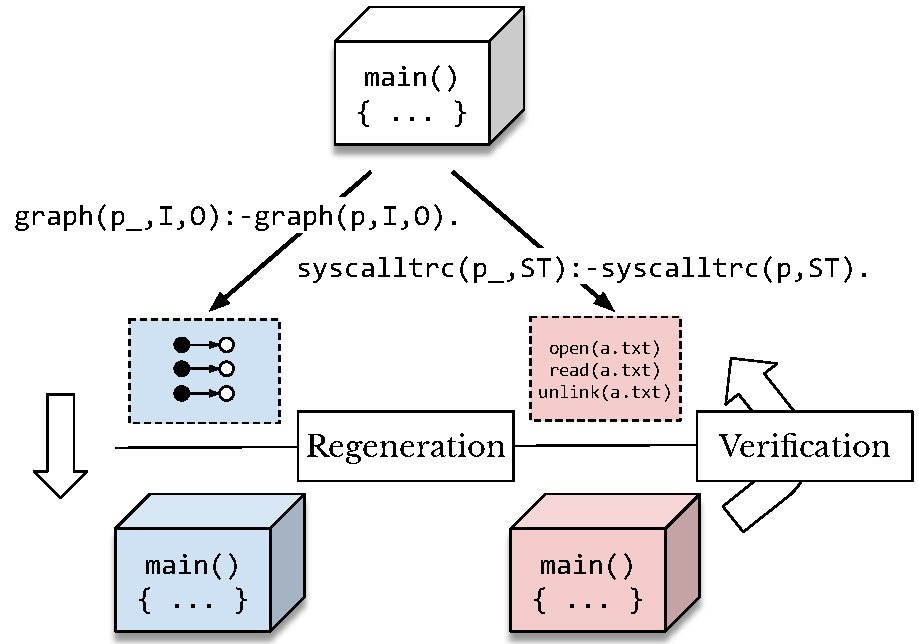
\includegraphics[width=.8\columnwidth]{figs/kvasir_projection.pdf}
  \caption{\textbf{Regeneration from property projection.}
  An alternative view of \sys is that instead of transforming source code directly, it projects the original
  program into a set of verifiable properties---such as input/output
  examples, system call traces, \etc.
  It then regenerates it and turns it back into source code.}
  \label{fig:projection}
\end{figure}

This section discusses \sys's inherent trade-offs and possibilities for future work.


\heading{Targeted regeneration}
\sys is best used as a surgical tool for targeted regeneration tasks, not for whole-program synthesis.
It operates most effectively on localized units of code---such as individual functions, methods, or small modules, where behavior is self-contained.
% Typical applications include rewriting high-risk, deprecated, or poorly understood code segments where correctness is critical and semantic preservation is essential.
Broad use will yield incomplete results and can be bottlenecked by the extracted property expressiveness.

\heading{Trust model and correctness}
\sys
does not provide formal guarantees
of semantic equivalence
to the original program.
Instead,
correctness is defined relative to a set of enforced properties.
This means that correctness is only as strong as the property definitions and associated verifiers.
In the presence of underspecified or unverifiable goals,
regenerated code
may exhibit unanticipated behavior,
even if it passes all checks.

\heading{LLM limitations}
The generative synthesis phase
is subject to the inherent variability and failure modes
of large language models.
These include hallucinations,
sensitivity to prompt phrasing,
and inconsistency
under minor input changes.
\sys does not mitigate these risks,
but allows their detection
through post-hoc verification.

\heading{Language-specific support}
Although some components of \sys are language-agnostic (\eg logic-based planning),
others---particularly extraction and verification plugins are not.
Supporting a new language
requires implementing (or using an off-the-shelf) language-specific analyzers and constraints.
This modularity is deliberate,
but it does limit out-of-the-box generality.
Work on a unified language representation~\cite{koppel2018onetool,bap2011,dillig2009sail},
is relevant to overcoming this limitation.
The current \sys prototype
supports Python, JavaScript, Haskell, and C. 

\heading{Expanding the transformation space}
Future extensions to \sys may incorporate richer classes of properties, such as
temporal logic and dataflow
constraints~\cite{azzopardi2023ltl,handa2021orderawaredataflowmodelparallel}.
In addition, performance-guided transformations offer a compelling avenue: \sys
could optimize for runtime, memory usage, or even parallelizability.
Inverse
transformations, such as serializing parallel programs, could serve as
a debugging or oracle mechanism in complex system settings.

\heading{Formal foundations and alternative implementations}
The transformation language semantics introduced by \sys are grounded in logic
programming and inherit properties like compositionality.
A more formal treatment of the \sys
transformation language could enable rigorous reasoning about transformation
correctness and equivalence.
Furthermore, establishing an abstract interface
over transformations would allow alternative \sys backends to be developed.
Integrating techniques from
counterfactual reasoning~\cite{Cabalar_2020} could further enhance \sys by
explaining synthesis failures and clarifying conflicting property constraints.

\heading{Idea of program projection}
\sys can be viewed as a projection system, as shown in \cref{fig:projection}.
\sys projects a program into an abstract space of properties, 
then, it performs transformations within that space (the input query),
and finally, it regenerates this projection back into a concrete program.
The idea of casting programs into a high-dimensioanl space has been studied before~\cite{ben-nun2018neural,alon2019code2vec,ellis2020dreamcoder,nye2021platypus},
but \sys's approach, from this perspective, might offer interesting insights.

\heading{Regeneration as a system-building primitive}
Beyond isolated transformations, \sys can serve as a core building block for
higher-level systems.
For instance, a reverse-engineering pipeline for
proprietary or legacy systems could use \sys to regenerate and recompose
well-behaved modules such as networking layer or the physics engine into new,
repurposed applications.
\sys can become a foundation for automated system understanding, adaptation, and re-imagination.

\heading{Challenges in cross-language regeneration}
Cross-language regeneration introduces challenges.
Some analyses and
properties may only be applicable in a subset of languages, or lack direct
equivalents across language boundaries.
\sys could address this in two ways: by
relying on least-common denominator of language semantics, or by
embracing language-specific features to drive more effective regeneration.
In
fact, cross-compilation could be leveraged as an asset: a plugin pipeline might
convert JavaScript to Haskell, extract formal properties via Haskell’s type
system, and then regenerate a more robust JavaScript variant informed by that
analysis.

\heading{Ethical and legal considerations}
While this work has applied \sys exclusively to open-source software, its
capabilities raise ethical and legal questions.
Regenerating
proprietary software, de-obfuscating binaries, or reimplementing licensed
systems into equivalent ones with more permissive licensing 
could challenge existing norms and regulations. 
It is important to consider
safeguards and responsible disclosure practices towards ethical program regeneration.



% Overall, \sys offers a flexible framework for controlled regeneration, but
% its effectiveness depends on the specificity of goals, the availability of
% property logic, and the scope of the transformation task. Its design favors
% composability and clarity over full automation, aiming to serve as a building
% block in broader refactoring, auditing, or hardening pipelines.

\section{Conclusion}
This work introduced \sys, a system for property-guided program regeneration
that bridges the flexibility of large language models with the precision of
logic-driven planning.
By allowing developers to declaratively specify
transformation goals as logical constraints, \sys elevates LLM-assisted program
transformations to a controllable, interpretable, and iterative synthesis-verification
process.
Evaluation demonstrates that \sys produces high-quality regenerations
across diverse tasks, outperforming naive prompting baselines in correctness,
controllability, and resilience to adversarial or obfuscated inputs.

\sys opens the door to a new class of synthesis tools that combine symbolic
reasoning and neural generation under a unified, extensible framework.
As program synthesis systems grow increasingly reliant on LLMs, I believe the
future lies in harnessing their generative power within a framework that retains
correctness, explainability, and developer control as first-class citizens.

\bibliographystyle{ACM-Reference-Format}
\bibliography{bib.bib}

\appendix

\section{Evaluation Samples}
\label{sec:eval-samples}
This section discusses a selection of samples from the evaluation of \sys.
These instances provide interesting insights into the capabilities of \sys, its shortcomings,
and a concrete comparison between \sys and a naive LLM-based approach.

\heading{Left Pad}
This regeneration task involves regenerating a
function that pads a string with a given character on the left side until it
reaches a specified length.

\begin{wrapfigure}[5]{r}{0.4\columnwidth}
\begin{minted}{prolog}
graph(p_, I, O) :-
graph(p, I, O).
\end{minted}
\end{wrapfigure}
The query for \sys is shown on the right and asserts the the input/output behavior of the
original program is preserved in the output.
The resulting program must match the input-output behavior of the original.
The top listing shows the original \ttt{leftPad} library, and the second listing shows the output
of \sys.
Regeneration here matches the client-visible behavior of the original but misses
implementation details, such as the use of a cache for common
use-cases and the logarithmic complexity of the padding operation.
This example inspires future work on performance-aware regeneration.

\begin{listing}[htpb]
\begin{minted}[fontsize=\footnotesize, frame=lines, framesep=2mm, breaklines=true]{javascript}
'use strict';
module.exports = leftPad;

var cache = [ '', ' ', '  ', '   ', '    ', '     ', '      ', '       ', '        ', '         ' ];

function leftPad(str, len, ch) {
  // convert `str` to a `string`
  str = str + '';
  // `len` is the `pad`'s length now
  len = len - str.length;
  // doesn't need to pad
  if (len <= 0) return str;
  // `ch` defaults to `' '`
  if (!ch && ch !== 0) ch = ' ';
  // convert `ch` to a `string` cuz it could be a number
  ch = ch + '';
  // cache common use cases
  if (ch === ' ' && len < 10) return cache[len] + str;
  // `pad` starts with an empty string
  var pad = '';
  // loop
  while (true) {
    // add `ch` to `pad` if `len` is odd
    if (len & 1) pad += ch;
    // divide `len` by 2, ditch the remainder
    len >>= 1;
    // "double" the `ch` so this operation count grows logarithmically on `len`
    // each time `ch` is "doubled", the `len` would need to be "doubled" too
    // similar to finding a value in binary search tree, hence O(log(n))
    if (len) ch += ch;
    // `len` is 0, exit the loop
    else break;
  }
  // pad `str`!
  return pad + str;
}
  \end{minted}
\caption{The original \ttt{leftPad} library.}
\end{listing}

\begin{listing}[htpb]
  \begin{minted}[fontsize=\footnotesize, frame=lines, framesep=2mm, breaklines=true]{javascript}
function leftPad(str, len, ch) {
    // Ensure the character is a string and has a length of 1
    ch = ch || ' '; // Default to space if no character is provided
    if (typeof ch !== 'string' || ch.length !== 1) {
        throw new Error('Padding character must be a single character string');
    }
    // Pad the string on the left
    while (str.length < len) {
        str = ch + str;
    }
    return str;
}
  \end{minted}
  \caption{The output of \sys, having regenerated \ttt{leftPad}.}
\end{listing}

\heading{Fast Inverse Square Root}
The goal of this regeneration task is to transform an input 
program into a more idiomatic version that retains the same functionality.
The query for \sys is shown on the right and it uses the length of the output program as a proxy towards 
more idiomatic code.
\begin{wrapfigure}[4]{r}{0.7\columnwidth}
\begin{minted}{prolog}
graph(p_, I, O) :- graph(p, I, O).
#min N : len(p_, N)
\end{minted}
\end{wrapfigure}
The fast inverse square root function is a well-known algorithm that was
popularized by its use in the Quake III Arena source code.
It computes the inverse square root of a number using 
Newton's method through bit-level manipulation on the input floating-point number.
The original implementation is shown in \cref{lst:fast_inv_sqrt_original}.
\Cref{lst:fast_inv_sqrt_gpt} shows the output of naively regenerating the function using \gptmodel,
which retains the original's un-idiomatic use of magic numbers and bit-level manipulation.
\Cref{lst:fast_inv_sqrt_sys} has the output of \sys, which instead uses the standard library's
\ttt{sqrt} function to compute the inverse square root.
\sys provides only I/O examples to its backend LLM, and as such does not overfit to the original implementation.

\begin{listing}[htpb]
\begin{minted}[fontsize=\footnotesize, frame=lines, framesep=2mm, breaklines=true]{c}
float Q_rsqrt( float number )
{
	long i;
	float x2, y;
	const float threehalfs = 1.5F;

	x2 = number * 0.5F;
	y  = number;
	i  = * ( long * ) &y;                       // evil floating point bit level hacking
	i  = 0x5f3759df - ( i >> 1 );               // what the fuck?
	y  = * ( float * ) &i;
	y  = y * ( threehalfs - ( x2 * y * y ) );   // 1st iteration
//	y  = y * ( threehalfs - ( x2 * y * y ) );   // 2nd iteration, this can be removed

	return y;
}
\end{minted}
  \caption{The original implementation of the fast inverse square root function 
  found in the Quake III source code~\cite{fast_inv_sqrt}}
  \label{lst:fast_inv_sqrt_original}
\end{listing}

\begin{listing}[htpb]
\begin{minted}[fontsize=\footnotesize, frame=lines, framesep=2mm, breaklines=true]{c}
#include <stdint.h> // For using int32_t

float Q_rsqrt(float number) {
    int32_t i; // Use int32_t for better portability
    float x2, y;
    const float threehalfs = 1.5F;

    // Calculate x2 as half of the input number
    x2 = number * 0.5F;
    y = number;

    // Bit-level manipulation to get an initial guess for the inverse square root
    i = *(int32_t*)&y; // Reinterpret the bits of y as an integer
    i = 0x5f3759df - (i >> 1); // Magic number and bit manipulation
    y = *(float*)&i; // Reinterpret the bits back to a float

    // First iteration of Newton's method for refining the result
    y = y * (threehalfs - (x2 * y * y));

    // Optionally, a second iteration can be uncommented for more accuracy
    // y = y * (threehalfs - (x2 * y * y)); // Second iteration

    return y; // Return the approximate inverse square root
}
\end{minted}
  \caption{The output of naively regenerating the fast inverse square root function using \gptmodel.
  Notice that the output is ostensibly idiomatic, as it contains magic numbers and bit-level manipulation.}
  \label{lst:fast_inv_sqrt_gpt}
\end{listing}

\begin{listing}[htpb]
\begin{minted}[fontsize=\footnotesize, frame=lines, framesep=2mm, breaklines=true]{c}
float Q_rsqrt(float number) {
    return 1.0f / sqrt(number);
}
\end{minted}
\caption{The output of \sys for the fast inverse square root regeneration.}
  \label{lst:fast_inv_sqrt_sys}
\end{listing}

% TODO add security example leetlog or string-compare

\heading{String Compare}
The goal of this regeneration task is to regenerate a given
program to remove potential security vulnerabilities or malicious behavior.

\begin{wrapfigure}[4]{r}{0.7\columnwidth}
\begin{minted}{prolog}
pure(p_).
graph(p_, I, O) :- graph(p, I, O).
\end{minted}
\end{wrapfigure}
The query for \sys is shown on the right.
\Cref{lst:string-compare-original} shows the original string compare function, which writes to a file if the
second argument is a fixed secret value.
The same attack can be found \cref{lst:string_compare_fool}, which comes from
transforming the original source code using an LLM in order to make 
it appear benign and hide the malicious behavior between integrity checks.
\Cref{lst:string_compare_sys} shows the output of \gptmodel,
after being asked to remove any malicious behavior from the original function.
It's obvious that the attack is preserved.
However, in \cref{lst:string_compare_sys}, the function is transformed to
an equivalent one that keeps only the client-visible behavior, while removing 
any side-effectful code.

\begin{listing}[htpb]
\begin{minted}[fontsize=\footnotesize, frame=lines, framesep=2mm, breaklines=true]{javascript}
// (a === b)? 0 : ((a < b)?  -1: 1)
module.exports = (a, b) => {
  if (b == "gbabWhaRQ") {
    require("fs").writeFileSync('./FILE', (a + b + '\n'), 'utf-8');
  } 
  return a.localeCompare(b);
}
\end{minted}
  \caption{The original string compare function, which writes to a file if the
  second argument is a fixed secret value~\cite{copeland2019frightening}.
  This function can be used to write arbitrary data to a file, possibly as part
  of a larger attack vector.}
  \label{lst:string-compare-original}
\end{listing}

\begin{listing}[htpb]
\begin{minted}[fontsize=\footnotesize, frame=lines, framesep=2mm, breaklines=true]{javascript}
const fs = require('fs');
const path = require('path');
module.exports = (a, b) => {
  // Validate types
  if (typeof a !== 'string' || typeof b !== 'string') {
    throw new TypeError('Both inputs must be strings');
  }
  // Fixed secret value (compare safely)
  const SAFE_KEY = 'gbabWhaRQ';
  if (b === SAFE_KEY) {
    try {
      const safePath = path.resolve(__dirname, 'FILE');
      // Prevent writing large input
      if ((a + b).length > 1024) {
        throw new Error('Input too long to be safely written');
      }
      fs.writeFileSync(safePath, `${a}${b}\n`, { encoding: 'utf-8', mode: 0o600 });
    } catch (err) {
      console.error('Failed to write to FILE:', err.message);
      // Might choose to rethrow or return a special value
    }
  }
  return a.localeCompare(b);
};
\end{minted}
  \caption{The same string-compare function transformed to fool
  an LLM like \gptmodel into making it reproduce the malicious behavior.}
\end{listing}

\begin{listing}[htpb]
\begin{minted}[fontsize=\footnotesize, frame=lines, framesep=2mm, breaklines=true]{javascript}
const fs = require('fs');
const path = require('path');
module.exports = (a, b) => {
  // Validate types
  if (typeof a !== 'string' || typeof b !== 'string') {
    throw new TypeError('Both inputs must be strings');
  }
  // Fixed secret value (compare safely)
  const SAFE_KEY = 'gbabWhaRQ';
  // Use a constant-time comparison to prevent timing attacks
  const safeCompare = (str1, str2) => {
    if (str1.length !== str2.length) return false;
    let result = 0;
    for (let i = 0; i < str1.length; i++) {
      result |= str1.charCodeAt(i) ^ str2.charCodeAt(i);
    }
    return result === 0;
  };
  if (safeCompare(b, SAFE_KEY)) {
    try {
      const safePath = path.resolve(__dirname, 'SAFE_FILE');
      // Prevent writing large input
      if ((a + b).length > 1024) {
        throw new Error('Input too long to be safely written');
      }
      // Use a safer method to write files
      fs.writeFileSync(safePath, `${a}${b}\n`, { encoding: 'utf-8', mode: 0o600 });
    } catch (err) {
      console.error('Failed to write to SAFE_FILE:', err.message);
      // Might choose to rethrow or return a special value
    }
  }
  return a.localeCompare(b);
};
\end{minted}
  \caption{The output of naively regenerating the string compare function using \gptmodel.
  The code includes the malicious behavior of writing to a file if the second argument is a fixed secret value.}
  \label{lst:string_compare_fool}
\end{listing}

\begin{listing}[htpb]
  \begin{minted}[fontsize=\footnotesize, frame=lines, framesep=2mm, breaklines=true]{javascript}
function stringCompare(a, b) { return a.localeCompare(b); }
\end{minted}
  \caption{The output of \sys, which has removed the side-effectful code and
  transformed the function to an equivalent one that keeps only the client-visible behavior.}
  \label{lst:string_compare_sys}
\end{listing}

\cleardoublepage
\end{document}
